\documentclass{article}

\usepackage[final]{nips_2018}

\usepackage[utf8]{inputenc} % allow utf-8 input
\usepackage[T1]{fontenc}    % use 8-bit T1 fonts
\usepackage{hyperref}       % hyperlinks
\usepackage{url}            % simple URL typesetting
\usepackage{booktabs}       % professional-quality tables
\usepackage{amsfonts}       % blackboard math symbols
\usepackage{nicefrac}       % compact symbols for 1/2, etc.
\usepackage{microtype}      % microtypography
\usepackage{graphicx}

\usepackage{array}
\usepackage{makecell}
\renewcommand\theadalign{bc}

\usepackage{natbib}
\bibliographystyle{unsrt}
\setcitestyle{square,numbers,sort}

\title{Word Embedding Aware Convolutional Networks for Sentiment Analysis}
\author{%
  Shrey Desai\\
  University of Texas at Austin\\
  \texttt{shreydesai@utexas.edu} \\
}

\begin{document}

\maketitle

\begin{abstract}
  Convolutional neural networks (CNNs) have become extremely popular models for text classification. Traditional architectures perform convolutions on dense vector representations of the input text, also known as \textit{word embeddings}. While researchers have explored various architectures to advance the state-of-the-art, the importance of the initial word embedding layer has not been considered as closely. This paper seeks to bridge this gap by empirically analyzing how using different word embeddings impact performance.\footnote{Code is available at \texttt{https://github.com/shreydesai/cnn-sentiment-analysis}}
\end{abstract}

\section{Introduction}

Convolutional neural networks (CNNs) have achieved impressive results in computer vision and speech recognition \cite{cv}. Recently, CNNs have overtaken traditional linear models in NLP for tasks such as text classification \cite{cnn_language}. These models leverage distributed representations of words---commonly referred to as \textit{word embeddings}---as their inputs. CNNs utilize linear filters that convolve across input regions to extract salient features. For text classification specifically, the filters learn to emphasize certain $n$-gram structures through backpropagation.

CNN architectures begin with a word embedding layer that replaces tokens with word vector representations, forming a sentence matrix. These vectors are either sampled from standard distributions or pre-populated using popular unsupervised algorithms. Depending on the method used, the vectors differ in their embedded syntactic and semantic information. This paper seeks to explore the impact of such variation, as most architectures do not consider using different word embeddings in the optimization process.

Using a sentence-level CNN similar to Kim's~\cite{kim}, we explore the effects of various word embedding initializations on sentiment analysis tasks. We consider embeddings obtained through a standard Gaussian, Word2vec, GloVe, and Numberbatch. The models are supervised on multiple sentiment datasets that contain "positive" and "negative" labels for sentences. In addition to reporting the performance, we also analyze how the models use the embeddings to make predictions.

\section{Model}

Each corpus is a collection of sentences with variable lengths. Let $V$ represent the vocabulary of the corpus. Sentences are encoded as a sequence $s = [s_1, s_2, \cdots, s_n]$ where $s_i \in V$. In order to create a uniform representation, we fix $n$ to represent the maximum sequence length. If $length(s) > n$, the first $n$ elements of the sequence are taken. If $length(s) < n$, the sequence is padded with a null symbol <PAD>. Consequently, <PAD> is not included in $V$.

The embedding layer functions as a lookup table that replaces each encoded item $s_i$ with a vector $\mathbf{w}_i \in \mathbb{R}^d$ that serves as the corresponding $d$-dimensional word embedding. The concatenation of $n$ word embedding vectors forms a sentence matrix $\mathbf{S} \in \mathbb{R}^{n \times d}$---the input to the CNN.

Next, we define a convolutional filter $\mathbf{W} \in \mathbb{R}^{h \times d}$ where $h$ represents the \textit{height} of the filter. The filter is not strided, padded, or dilated. Let $\mathbf{S}[i:j]$ represent a sub-matrix of $\mathbf{S}$ from rows $i$ through $j$ inclusive. The feature map $\mathbf{c} \in \mathbb{R}^{n - h + 1}$ is created by applying the filter to each possible window of $h$ words, using a non-linear function $f$ and bias $b \in \mathbb{R}$:

\begin{equation}
    \mathbf{c} = \sum_{i=1}^{n-h+1} f(\mathbf{S}[i:i+h] \cdot \mathbf{W} + b)
\end{equation}

\textit{1-max pooling}~\cite{pooling}, defined as $\hat{c} = \max \{\mathbf{c}\}$, picks the maximum scalar from the feature map. This allows us to (a) propagate the maximum signal further into the network, (b) reduce the dimension of the input, and (c) introduce additional non-linearities.

We define a single $n$-gram block as consisting of a convolutional and pooling layer, as described above. Our network uses multiple $n$-gram blocks---the height of each filter is varied across the blocks, so the CNN learns multiple $n$-gram representations from the input. The outputs of these $n$-gram blocks are concatenated, then fed into a fully connected layer. For regularization we use a dropout layer that stochastically disables neurons to force them to learn independently useful features.

Softmax converts the fully connected layer output $\mathbf{x} \in \mathbb{R}^K$ into a distribution $\mathbf{y}$ over the $K$ classes:

\begin{equation}
    P(\mathbf{y}|\mathbf{x}) = \frac{\exp (\mathbf{x})}{\sum_{j=1}^K \mathbf{x}_j}
\end{equation}

Finally, we use binary cross-entropy loss as the objective function since we have two classes to categorize sentiment---positive and negative.

\section{Experiments}

\subsection{Datasets}

\begin{table}
    \caption{Statistics of datasets after preprocessing. $l$: Average sentence length. $|V|$: Vocabulary size. $|V_1|$,$|V_2|$,$|V_3|$: Counts of words that appear in the pre-trained Word2vec, GloVe, and Numberbatch embeddings, respectively. \textit{Train}: Number of training samples. \textit{Test}: Number of testing samples; $10$-fold cross-validation (CV) is used if a testing set is not available.}
    \label{datasets-table}
    \centering
    \begin{tabular}{llllllll}
        \toprule
        & \multicolumn{1}{c}{$l$} & \multicolumn{1}{c}{$|V|$} & \multicolumn{1}{c}{$|V_1|$} & \multicolumn{1}{c}{$|V_2|$} & \multicolumn{1}{c}{$|V_3|$} & \multicolumn{1}{c}{\textit{Train}} & \multicolumn{1}{c}{\textit{Test}} \\
        \midrule
        MR & 115 & 18766 & 16448 & 17614 & 16914 & 9595 & CV \\
        SST-2 & 872 & 16238 & 14829 & 15849 & 15268 & 6920 & 1821 \\
        MPQA & 18 & 6249 & 6083 & 6189 & 6128 & 9544 & CV \\
        \bottomrule
    \end{tabular}
\end{table}

We test our models on several datasets. The datasets are summarized as follows: (1) \textbf{MR:} Sentence polarity dataset (Pang and Lee)~\cite{panglee}. (2) \textbf{SST-2:} Stanford Sentiment Treebank. Adapted from SST-1, which contained fine-grained labels (very positive, positive, neutral, negative, very negative), but this version has binary labels only with neutral sentences removed (Socher et al.)~\cite{socher}. (3) \textbf{MPQA:} Opinion polarity dataset from the Multi-Perspective Question Answering corpus (Wiebe et al.)~\cite{wiebe}. Further dataset information is detailed in Table~\ref{datasets-table}.

\subsection{Hyperparameters}
For all datasets, we define the maximum sequence length as the average sentence length, use word embedding dimensions of $300$, and do not modify the original vocabulary. The CNN is constructed with three $n$-gram blocks of filter sizes $3$, $4$, and $5$, respectively, with $128$ channels each. ReLU~\cite{relu}, defined as $y=\max(0,x)$, is used as the non-linear activation function. The model is trained for $30$ epochs using the Adam~\cite{adam} optimizer, learning rate of $1{\rm e}{-3}$, no weight decay, dropout rate of $0.5$, and a mini-batch size of $32$. Early stopping is used to select checkpointed models with the highest accuracies on the validation sets. These hyperparameters were chosen through a minimal grid search on the MR dataset.

\subsection{Model Variations}
Using a standard text CNN as a base model, we define several variations by experimenting with different types of embedding layers:
\begin{itemize}
    \item \textbf{CNN-random:} Embeddings are randomly initialized through a standard Gaussian.
    \item \textbf{CNN-word2vec:} Embeddings are initialized with Word2vec~\cite{w2v}. Word2vec describes a family of unsupervised neural language models that predict the linguistic context of words in a corpus. We use Mikolov et al.'s embeddings trained on 300 million words from Google News with a continuous bag-of-words model.
    \item \textbf{CNN-glove:} Embeddings are initialized with GloVe~\cite{glove}. GloVe is an unsupervised algorithm that finds co-occurrence statistics from a global word-word co-occurrence matrix. We use Pennington et al.'s embeddings trained on the Wikipedia 2014 dump and Gigaword 5.
    \item \textbf{CNN-numberbatch:} Embeddings are initialized with Numberbatch~\cite{nb}. Numberbatch is an ensemble method that combines data from ConceptNet 5.5, Word2vec, GloVe, and Open Subtitles 2016~\cite{opensub}. We use Speer et al.'s English-only embeddings (version 16.04).
\end{itemize}

The embeddings used in each model have a dimensionality of $300$. Further, for words that do not have entries in the pre-trained embeddings, their corresponding word vectors are randomly initialized from a standard Gaussian.


\section{Discussion}

\subsection{Results}

\begin{figure}
  \centering
  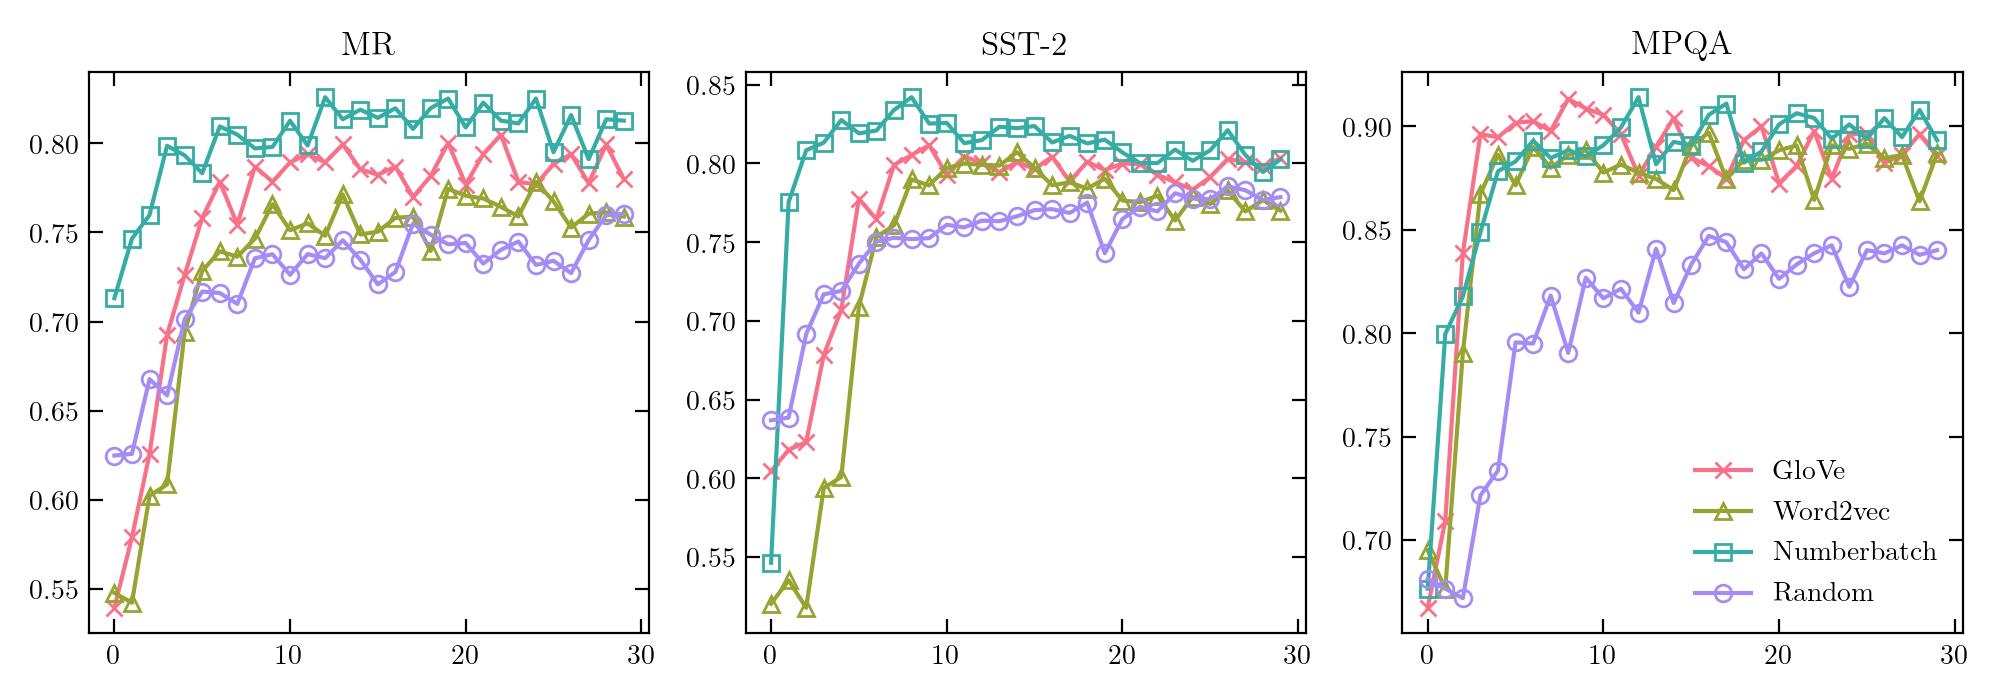
\includegraphics[width=5in]{validation.png}
  \caption{Validation accuracies of the models across training epochs.}
  \label{fig:validation}
\end{figure}

The validation accuracies are visualized in Figure~\ref{fig:validation}. Models with random embeddings perform consistently worse than models with pre-trained embeddings. The MPQA dataset especially shows a large drop-off in performance when using random embeddings. The model accuracies are closer together for the MR and SST-2 datasets, but the pre-trained embedding models still perform better than the random embedding models. These conclusions are also consistent with the test accuracies detailed in Table~\ref{test-table}. 

The results cohere with the idea that models with random embeddings require more epochs to train, converge to suboptimal minima, and suffer from low accuracies. In contrast, models with pre-trained embeddings collectively perform well. In particular, they converge rapidly to a more optimal solution. For example, the Numberbatch models converge in about 10 epochs as opposed to the random models which converge in 20-30 epochs while maintaining strong accuracies.

When comparing the pre-trained embedding models, the Numberbatch models seem to perform the best. Numberbatch models achieve the highest accuracies on the MR and SST-2 datasets, but get slightly edged out by the GloVe model on the MPQA dataset. These results are intuitive---the Numberbatch embeddings are created through an ensemble of other pre-trained embeddings, so they maximize the efficacy of each individual embedding.

\begin{table}
    \caption{Test accuracies of the models.}
    \label{test-table}
    \centering
    \begin{tabular}{llll}
        \toprule
        & \multicolumn{1}{c}{MR} & \multicolumn{1}{c}{SST-2} & \multicolumn{1}{c}{MPQA} \\
        \midrule
        CNN-random & 0.739 & 0.777 & 0.817 \\
        CNN-word2vec & 0.757 & 0.823 & 0.859 \\
        CNN-glove & 0.778 & 0.824 & \textbf{0.885} \\
        CNN-numberbatch & \textbf{0.794} & \textbf{0.846} & 0.876 \\
        \bottomrule
    \end{tabular}
\end{table}

\subsection{Semantic Analysis}

\begin{table}
    \caption{Top 4 neighboring words across SST-2 models.}
    \label{neighbor-table}
    \centering
    \begin{tabular}{lllll}
        \toprule
        & \multicolumn{1}{c}{Random} & \multicolumn{1}{c}{Word2vec} & \multicolumn{1}{c}{GloVe} & \multicolumn{1}{c}{Numberbatch} \\
        \midrule
        good & \makecell{\textit{<PAD>} \\ \textit{dumbest} \\ \textit{fidgeted} \\ \textit{moral}} & \makecell{\textit{nice} \\ \textit{excellent} \\ \textit{decent} \\ \textit{great}} & \makecell{\textit{great} \\ \textit{excellent} \\ \textit{decent} \\ \textit{nice}} & \makecell{\textit{better} \\ \textit{well} \\ \textit{always} \\ \textit{excellent}} \\
        \midrule
        n't & \makecell{\textit{<PAD>} \\ \textit{atrociously} \\ \textit{introspective} \\ \textit{discovering}} & \makecell{\textit{no} \\ \textit{not} \\ \textit{nothing} \\ \textit{neither}} & \makecell{\textit{lisa} \\ \textit{ca} \\ \textit{os} \\ \textit{ritchie}} & \makecell{\textit{do} \\ \textit{did} \\ \textit{not} \\ \textit{know}} \\
        \midrule
        , & \makecell{\textit{<PAD>} \\ \textit{limply} \\ \textit{boisterous} \\ \textit{unfulfilled}} & \makecell{\textit{of} \\ \textit{and} \\ \textit{recent} \\ \textit{our}} & \makecell{\textit{disconnects} \\ \textit{overtly} \\ \textit{abrasive} \\ \textit{apex}} & \makecell{\textit{.} \\ \textit{and} \\ \textit{but} \\ \textit{though}} \\
        \bottomrule
    \end{tabular}
\end{table}


To further understand why certain embeddings perform better than others, we test the embeddings' abilities to predict context. We search for the top neighboring words for "good", "n't", and "," using Euclidean distance in the word embedding layers of SST-2 models; the results are shown in Table~\ref{neighbor-table}. It is immediately apparent that the random embedding model is unable to predict the context of words. The neighboring words in the random embedding model carry no relevance to the original words.

In contrast, the pre-trained embedding models generally perform better. For "good", the pre-trained embedding models produce similar neighboring words. However, the results are mixed for "n't" and ",". The GloVe model is unable to recognize the context in which "n't" and "," appear, while the Word2vec model gives slightly more convincing results. The Numberbatch model is unequivocally the best as it recognizes the context of contractions, determiners, and connectives.

The syntactic and semantic information stored in word embeddings is therefore strongly linked to performance. Intuitively speaking, words that cluster together in a vector space receive similar weights from a convolutional filter. This is because there is lower variability among the vectors of a cluster in comparison to the vectors of another cluster. This principle can be exploited in sentiment analysis tasks since positive and negative words often cluster together---these words can easily be used to predict subjectivity in a text.

Figure~\ref{fig:filter} empirically verifies this claim. Most notably, the filter learns to emphasize positive trigrams such as "visually stunning rumination". Further, it does not weight trigrams with function words---"the", "and", "on", "between"---as much since these words are not representative of a sentence's sentiment. Convolutions are location invariant operations by nature, so the filter is able to weight the trigrams correctly irrespective of where they appear in the sentence.

\begin{figure}
  \centering
  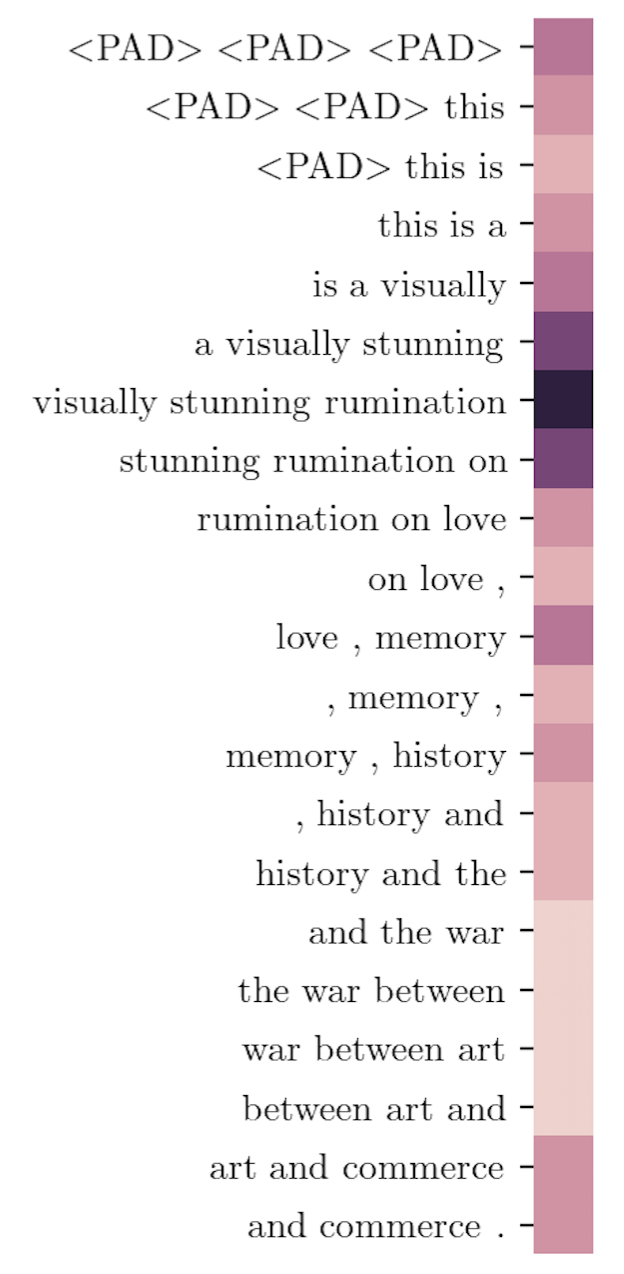
\includegraphics[width=2in]{filter.png}
  \caption{Heatmap of the weights a trigram convolutional filter assigns to the tokens of a sentence. Darker colors imply higher weights while lighter colors imply lower weights. The visualization is generated from a Numberbatch embedding model trained on SST-2.}
  \label{fig:filter}
\end{figure}

\section{Conclusion}
Word embeddings have a significant impact on CNN performance. We show that models with random embeddings consistently perform worse than models with pre-trained embeddings. Pre-trained embeddings capture syntactic and semantic information about a corpus that deep learning models use to make classification decisions. CNNs exploit the fact that semantically similar words cluster together in low-dimensional spaces. 

In particular, we show that the Numberbatch embedding models have faster training times and convergence than Word2vec and Glove embedding models. This is primarily attributed to the Numberbatch embeddings' ability to best predict the linguistic context of words. Further, the model fine tunes the embeddings during the training process, leading to better performance over time.

For future work, there are a couple of things we can do. First, we could try using different datasets---the ones used in our experiments were quite small. Second, we primarily focus on sentence-level sentiment analysis tasks, but we can also expand to other forms of text classification. Third, it would be interesting to see if our results differ for deeper convolutional architectures.

{\small
\bibliographystyle{ieee}
\bibliography{egbib}
}

\end{document}